\documentclass[a5paper, 10pt]{tekst}

\usepackage{titlesec}
\usepackage{indentfirst}

\begin{document}
	\thispagestyle{empty}
	\onehalfspacing
	\titleformat*{\section}{\sffamily\bfseries}
	\sffamily
	
	\begin{center}
		\Huge \p{\f{壁}{かべ}の}\p{\f{穴}{あな}}、\p{\f{第}{だい}}\p{\f{四}{よん}\f{話}{わ}}
	\end{center}
	
	\begin{figure}[h]
		\centering
		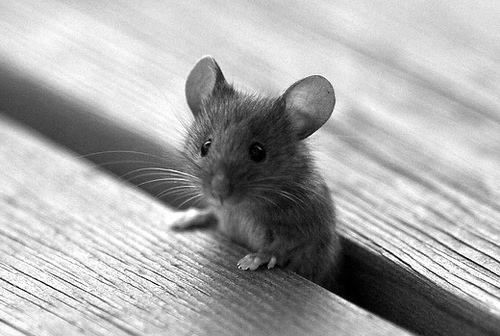
\includegraphics[width=0.5\linewidth]{figures/ねずみ5.jpg}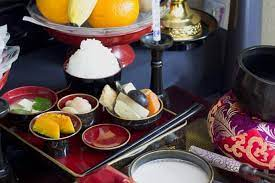
\includegraphics[width=0.5\linewidth]{figures/ねずみ7.jpeg}
	\end{figure}
	
	{\Large\sloppy
		\noindent「クミコ~ 、 お \ruby{仏壇}{ぶつだん}の お \ruby{水}{みず}と ご\ruby{飯}{はん}を \ruby{交換}{こうかん} して ちょうだい」 と、 また クミコの \ruby{母}{かあ}ちゃんの \ruby{声}{こえ}が した。クミコは \ruby{不機嫌}{ふきげん}そうに、「 ちょっと \ruby{待}{ま}ってよー。 あと、 \ruby{少}{すこ}しだけ~」 と \ruby{言}{い}って、 \ruby{座布団}{ざぶとん}の \ruby{上}{うえ}で ゴロゴロ していた。  
		
		\noindent  クミコの \ruby{家}{いえ}では、 \ruby{仏様}{ほとけさま}に、 \ruby{毎朝}{まいあさ}、 お \ruby{水}{みず}と ご\ruby{飯}{はん}を お\ruby{供}{そな}え していた。 それを \ruby{交換}{こうかん} するのは、 クミコの \ruby{仕事}{しごと} だった。 そう、 この お\ruby{供}{そな}え \ruby{物}{もの}の \ruby{炊}{た}きたての ご\ruby{飯}{はん}が、 モチモチ していて、 \ruby{最高}{さいこう}に おいしいん だ。 \ruby{仏様}{ほとけさま}には \ruby{申}{もう}し\ruby{訳}{わけ}ないと \ruby{思}{おも}っているよ。 でも、 \ruby{僕}{ぼく}\ruby{達}{たち} \ruby{家族}{かぞく}は、 \ruby{毎朝}{まいあさ}、 それを ちょっとだけ もらって \ruby{食}{た}べるのを、 \ruby{楽}{たの}しみに していた。 
		
		\noindent \ruby{仏様}{ほとけさま}には、 \ruby{昨日}{きのう}から お まんじゅうが お\ruby{供}{そな}え して あった。 しかし、 \ruby{僕}{ぼく}\ruby{達}{たち}は、 \ruby{目立}{めだ}つ \ruby{物}{もの}は \ruby{盗}{ぬす}んでは いけないと \ruby{教}{おし}えられていた。 \ruby{僕}{ぼく}\ruby{達}{たち}が \ruby{盗}{ぬす}んだ ことが、 \ruby{人間}{にんげん}に バレては いけないから だ。 ご\ruby{飯}{はん}は、 \ruby{家族}{かぞく} 4\ruby{匹}{ひき}で \ruby{食}{た}べられる \ruby{量}{りょう}だけを もらうん だ。 でも、 ご\ruby{飯}{はん}が \ruby{大盛}{おおも}りの \ruby{日}{ひ}は、 \ruby{少}{すこ}しだけ \ruby{多}{おお}めに もらっても \ruby{良}{よ}かった。 
		
	}\clearpage
	\titleformat*{\section}{\rmfamily\bfseries}
	\rmfamily
	
	\section*{Vokabular}
	\begin{multicols}{2}[\centering\textbf{Bitno}]\noindent
		\dictentry{交換}{こうかん}{\item zamjena,razmjena}{imenica, suru-glagol}
		\dictentry{不機嫌}{ふきげん}{\item nezadovoljstvo}{imenica, na-pridjev}
		\dictentry{炊きたて}{たきたて}{\item svježe skuhano}{no-pridjev}
		\dictentry{最高}{さいこう}{\item najbolji}{imenica, no-pridjev, na-pridjev}
		\dictentry{申し訳ない}{もうしわけない}{\item ispričavam se}{fraza, i-pridjev}
		\dictentry{盗む}{ぬすむ}{\item ukrasti}{glagol (五)}
		\dictentry{量}{りょう}{\item količina}{imenica}
		\dictentry{大盛り}{おおもり}{\item velika porcija}{imenica}
		\dictentry{多め}{おおめ}{\item povrh, još i više (količinski)}{imenica, no-pridjev, na-pridjev}
	\end{multicols}
	
	\begin{multicols}{2}[\centering\textbf{Ostalo}]
		\dictentry{仏壇}{ぶつだん}{\item Budistički oltar (kućni)}{imenica}
		\dictentry{水}{みず}{\item voda}{imenica}
		\dictentry{ご飯}{ごはん}{\item objed, kuhana riža}{imenica}
		\dictentry{母ちゃん}{かあちゃん}{\item mama}{imenica}
		\dictentry{待つ}{まつ}{\item čekati}{glagol (五)}
		\dictentry{少し}{すこし}{\item malo (količinski)}{imenica, prijedlog}
		\dictentry{言う}{いう}{\item reći}{glagol (五)}
		\dictentry{座布団}{ざぶとん}{\item jastuk}{imenica}
		\dictentry{上}{うえ}{\item iznad}{imenica, no-pridjev, prilog}
		\dictentry{家}{いえ}{\item kuća}{imenica}
		\dictentry{仏様}{ほとけさま}{\item Buda}{imenica}
		\dictentry{毎朝}{まいあさ}{\item svako jutro}{imenica, prilog}
		\dictentry{供える\footnotemark}{そなえる}{\item ponuditi}{glagol (一)}
		\dictentry{仕事}{しごと}{\item posao}{imenica}
		\dictentry{物}{もの}{\item stvar}{imenica}
		\dictentry{思う}{おもう}{\item misliti}{glagol (五)}
		\dictentry{僕達}{ぼくたち}{\item mi}{zamjenica}
		\dictentry{家族}{かぞく}{\item obitelj}{imenica}
		\dictentry{食べる}{たべる}{\item jesti}{glagol (一)}
		\dictentry{楽しみにする}{たのしみにする}{\item veseliti se}{suru-glagol}
		\dictentry{昨日}{きのう}{\item jučer}{imenica}
		\dictentry{目立つ}{めだつ}{\item isticati se, odstupati}{glagol (五)}
		\dictentry{教える}{おしえる}{\item poučavati, reći}{glagol (一)}
		\dictentry{人間}{にんげん}{\item čovjek}{imenica}
		\dictentry{4匹}{よんひき}{\item 4 male životinje}{brojač}
		\dictentry{日}{ひ}{\item dan}{imenica}
		\dictentry{良い}{よい}{\item dobro}{i-pridjev}
	\end{multicols}
        \footnotetext{U tekstu ovaj glagol čudno izgleda zato što je stavljen u svoju pristojniju verziju koja je dio keiga i tvori se tako da se ispred korjena glagola stavi お ili ご, a iza se stavi glagol する u odgovarajućem obliku.}
	
	\clearpage
	
	\section*{Domaća zadaća}
	\begin{enumerate}
		\item Napišite kratku priču ili par rečenica koristeći riječi iz kutije ispod.
		Rečenice ili tekst ne moraju nužno biti vezane uz sam tekst.
		\begin{center}
			\vspace{0.5em}
			\fbox{交換 ・ 不機嫌 ・ 最高 ・ 盗む ・ 多め}\vspace{1.4em}
			\rule{\linewidth}{0.5pt}\\[0.6em]
			\rule{\linewidth}{0.5pt}\\[0.6em]
			\rule{\linewidth}{0.5pt}\\[0.6em]
			\rule{\linewidth}{0.5pt}\\[0.6em]
			\rule{\linewidth}{0.5pt}\\[0.6em]
			\rule{\linewidth}{0.5pt}\\[0.6em]
			\rule{\linewidth}{0.5pt}
		\end{center}
		
		\item Odgovorite na pitanja:
		\begin{enumerate}[label=(\roman*)]
			\raggedright
			\item\vspace{0.5em}\p{クミコの}\p{\f{家}{いえ}で}\p{\f{毎日}{まいにち}}\p{何を}\p{して}\p{いるのですか?}
			\rule{\linewidth}{0.5pt}\\[0.6em]
			\rule{\linewidth}{0.5pt}
			\item\vspace{0.5em}\p{クミコの}\p{\f{仕事}{しごと}は}\p{\f{何}{なん}ですか?}
			\rule{\linewidth}{0.5pt}\\[0.6em]
			\rule{\linewidth}{0.5pt}
			\item\vspace{0.5em}\p{\f{家族}{かぞく}は}\p{何を}\p{\f{楽}{たの}しみに}\p{して}\p{いました?}
			\rule{\linewidth}{0.5pt}\\[0.6em]
			\rule{\linewidth}{0.5pt}
			\item\vspace{0.5em}\p{\f{語}{かた}り}\p{\f{手}{て}は}\p{\f{何}{なん}の}\p{\f{食}{た}べ}\p{\f{物}{もの}を}\p{\f{盗}{ぬす}んでは}\p{いけないのですか?}\p{なぜですか?}
			\rule{\linewidth}{0.5pt}\\[0.6em]
			\rule{\linewidth}{0.5pt}
			\item\vspace{0.5em}\p{\f{家族}{かぞく}は}\p{どのくらい}\p{\f{ご飯}{はん}を}\p{\f{盗}{ぬす}むのですか?}
			\rule{\linewidth}{0.5pt}\\[0.6em]
			\rule{\linewidth}{0.5pt}
			\item\vspace{0.5em}\p{いつも}\p{\f{同}{おな}じ}\p{\f{量}{りょう}を}\p{\f{盗}{ぬす}むのですか?}
			\rule{\linewidth}{0.5pt}\\[0.6em]
			\rule{\linewidth}{0.5pt}
		\end{enumerate}		
		\item Nadopunite sljedeće rečenice riječima iz kutije ispod:
		\begin{center}
			\choicebox{交換した ・ 不機嫌 ・ 炊きたて ・ 最高 ・ 申し訳ない\\盗まれた|盗む ・ 大量 ・ 大盛り ・ 多め}
		\end{center}
		\begin{enumerate}[label=(\roman*)]
			\raggedright
			
			\vspace{0.5em}\item \p{\ansline{}の}\p{プレゼントを}\p{\f{用意}{ようい}}\p{するから}\p{\f{楽}{たの}しみに}\p{してて。}
			\item \p{\f{花子}{はなご}ちゃんは}\p{\f{今日}{きょう}\ansline{}だから}\p{\f{武}{たけし}\f{君}{くん}が}\p{ぼこぼこに}\p{された。}
			\item \p{ほか}\p{ほかの\ansline{}}\p{\f{ご飯}{はん}が}\p{\f{食}{た}べたい。}
			\item \p{\f{私}{わたくし}は}\p{\f{古}{こ}}\p{\f{新聞}{しんぶん}をちり}\p{\f{紙}{がみ}と\ansline{}。}
			\item \p{お}\p{\f{茶}{ちゃ}の}\p{\f{葉}{は}は}\p{もう}\p{\f{少}{すこ}し\ansline{}に}\p{\f{入}{い}れた}\p{ほうが}\p{\f{美味}{おい}しいですよ。}
			\item \p{\ansline{}}\p{けど}\p{今}\p{あの}\p{\f{子}{こ}は}\p{\f{出}{で}かけて}\p{いるの。}
			\item \p{\f{鈴木}{すずき}さんは}\p{\f{下着}{したぎ}を\ansline{}}\p{\f{変態}{へんたい}が}\p{\f{大嫌}{だいきら}いだ、}\p{それは}\p{\f{小}{ちい}さい}\p{ころ}\p{\f{下着}{したぎ}を}\p{たくさん\ansline{}から。}
			\item \p{\f{警察}{けえいさつ}は}\p{\f{学校}{がっこう}で\ansline{}の}\p{\f{薬物}{やくぶつ}を}\p{\f{押収}{おうしゅう}}\p{した。}
			\item \p{この\ansline{}の}\p{ラーメンは}\p{\f{量}{りょう}が}\p{\f{多}{おお}すぎで、}\p{\f{食}{た}べ}\p{きれない。}
		\end{enumerate}
	\end{enumerate}
\end{document}